\documentclass[10pt]{article}
\usepackage[UTF8]{ctex}

\usepackage[utf8]{inputenc} % allow utf-8 input

\usepackage{amsmath,amscd}
\usepackage{amssymb,array}
\usepackage{amsfonts,latexsym}
\usepackage{graphicx,subfig,wrapfig}
\usepackage{times}
\usepackage{psfrag,epsfig}
\usepackage{verbatim}
\usepackage{tabularx}
\usepackage[pagebackref=true,breaklinks=true,letterpaper=true,colorlinks,bookmarks=false]{hyperref}
\usepackage{cite}
\usepackage{algorithm}
\usepackage{multirow}
\usepackage{caption}
\usepackage{algorithmic}
\usepackage[amsmath,thmmarks]{ntheorem}
\usepackage{listings}
\usepackage{color}


\newtheorem{thm}{Theorem}
\newtheorem{mydef}{Definition}

\DeclareMathOperator*{\rank}{rank}
\DeclareMathOperator*{\trace}{trace}
\DeclareMathOperator*{\acos}{acos}
\DeclareMathOperator*{\argmax}{argmax}


\renewcommand{\algorithmicrequire}{ \textbf{Input:}}     
\renewcommand{\algorithmicensure}{ \textbf{Output:}}
\renewcommand{\mathbf}{\boldsymbol}
\newcommand{\mb}{\mathbf}
\newcommand{\matlab}[1]{\texttt{#1}}
\newcommand{\setname}[1]{\textsl{#1}}
\newcommand{\Ce}{\mathbb{C}}
\newcommand{\Ee}{\mathbb{E}}
\newcommand{\Ne}{\mathbb{N}}
\newcommand{\Se}{\mathbb{S}}
\newcommand{\norm}[2]{\left\| #1 \right\|_{#2}}

\newenvironment{mfunction}[1]{
	\noindent
	\tabularx{\linewidth}{>{\ttfamily}rX}
	\hline
	\multicolumn{2}{l}{\textbf{Function \matlab{#1}}}\\
	\hline
}{\\\endtabularx}

\newcommand{\parameters}{\multicolumn{2}{l}{\textbf{Parameters}}\\}

\newcommand{\fdescription}[1]{\multicolumn{2}{p{0.96\linewidth}}{
		
		\textbf{Description}
		
		#1}\\\hline}

\newcommand{\retvalues}{\multicolumn{2}{l}{\textbf{Returned values}}\\}
\def\0{\boldsymbol{0}}
\def\b{\boldsymbol{b}}
\def\bmu{\boldsymbol{\mu}}
\def\e{\boldsymbol{e}}
\def\u{\boldsymbol{u}}
\def\x{\boldsymbol{x}}
\def\v{\boldsymbol{v}}
\def\w{\boldsymbol{w}}
\def\N{\boldsymbol{N}}
\def\X{\boldsymbol{X}}
\def\Y{\boldsymbol{Y}}
\def\A{\boldsymbol{A}}
\def\B{\boldsymbol{B}}
\def\y{\boldsymbol{y}}
\def\cX{\mathcal{X}}
\def\transpose{\top} % Vector and Matrix Transpose

%\long\def\answer#1{{\bf ANSWER:} #1}
\long\def\answer#1{}
\newcommand{\myhat}{\widehat}
\long\def\comment#1{}
\newcommand{\eg}{{e.g.,~}}
\newcommand{\ea}{{et al.~}}
\newcommand{\ie}{{i.e.,~}}

\newcommand{\db}{{\boldsymbol{d}}}
\renewcommand{\Re}{{\mathbb{R}}}
\newcommand{\Pe}{{\mathbb{P}}}

\hyphenation{MATLAB}

\usepackage[margin=1in]{geometry}

\begin{document}
	
\title{	Numerical Optimization, 2020 Fall\\Homework 1}
\author{Tao Huang\\2018533172}
\date{Due on 14:59 Sep 15, 2020
	}
\maketitle

%%%%%--------------------
\section{优化问题的应用}
\Large{给出目前业界线性规划的一个应用场景.介绍模型(变量、约束、目标).一般的规模是多大?}\\\\
\Large{\textbf{解:}}
\begin{itemize}
\item 应用场景:发电企业需要在满足发电量的情况下尽可能减小煤炭采购的成本
\item 模型描述: 某发电企业管理$n$个燃煤电厂,当月总
发电量目标为$ G $;可从$ m $个煤矿采购煤炭 ;$a_i$ 为第 $i$ 个
煤矿的最大供应能力,$d_j$ 为第 $j$ 个电厂的供电煤耗,$f_j$ 为
第 $j$ 个电厂当月的最大发电能力[$i=1,2,...,m;j=1,2,...,n;
(i, j)$ 代表一对供需组合];从第$ i $个煤矿到第$ j $个电厂的
采购成本为$ c_{ij}$
\item 优化变量:每对供需组合的运输量$x_{ij}$
\item 目标函数:使该企业的总采购成本$Z$最小,即$\min Z=\sum_{i=1}^m\sum_{j=1}^n c_{ij}x_{ij}$。
\item 优化约束:
\begin{itemize}
\item [1.] 不突破每个煤矿的供应能力,$\sum_{j=1}n_{ij}\le a_i$;
\item [2.] 各电厂的发电量不突破当月发电能力,$d_j\sum_{i=1}^mx_{ij}\le f_j$;
\item [3.] 满足总发电量目标,$\sum_{j=1}^n(d_j\sum_{i=1}^mx_{ij})=G$;
\item [4.] 采购量非负,$x_{ij}\ge 0$.
\end{itemize}
\item 一般规模:该模型的规模由电厂和煤矿的数量决定(即i,j的离散取值总对数),因此在实际中的规模大致在$10^1-10^2$数量级范围内。
\end{itemize}
Reference: 田森.基于线性规划技术的发电量—燃煤成本模型研究[J].企业管理,2017(S2):249-251.
\section{将下述问题建模成线性规划问题} 

一个原油精练场有8百万桶原油A和5百万桶原油B用以安排下个月的生产.可用这些资源来生产售价为38元/桶的汽油,或者生产售价为33元/桶的民用燃料油.有三种生产过程可供选择,各自的生产参数如下:
\begin{figure}[ht]
	\centering
	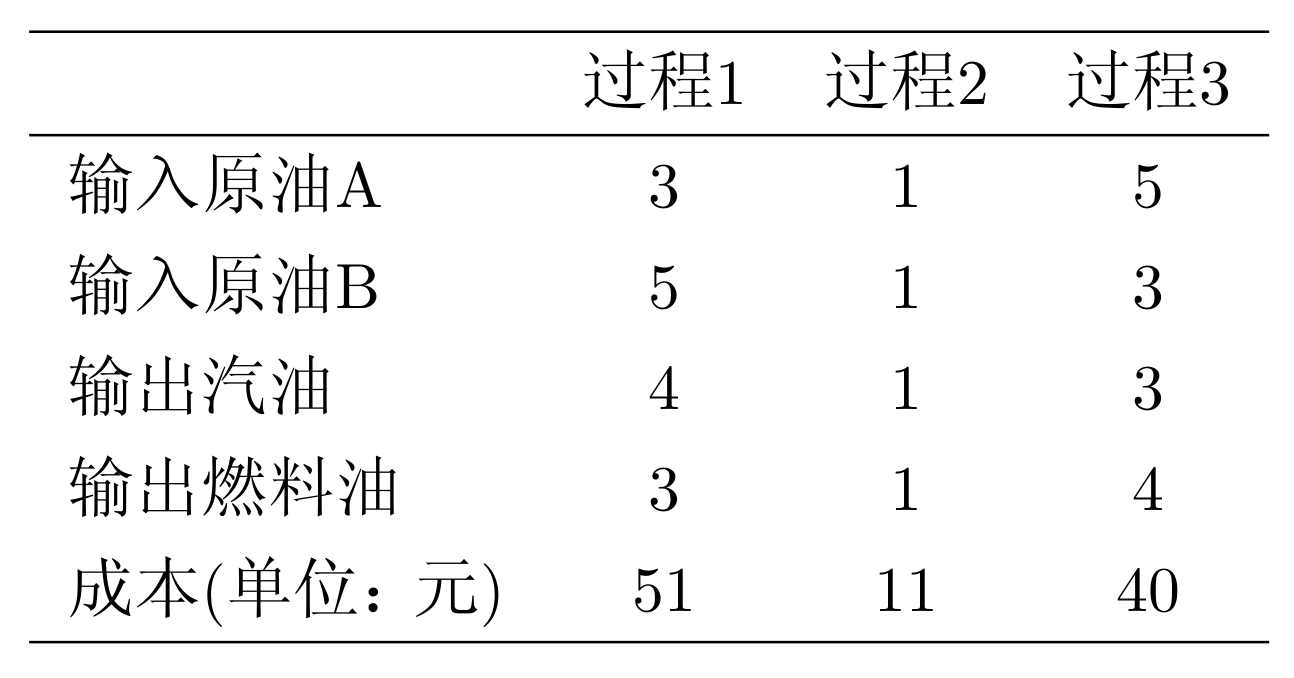
\includegraphics[width=0.5\linewidth]{prob1.png}
	%\caption{Accuracy demo.}
	\label{fig.prob1}
\end{figure}
除成本外,所有的量均以桶为单位.例如,对于第一个过程而言,利用3桶原油A和5桶原油B可以生产4桶汽油和3桶民用燃料油,成本为51元.表格中的成本指总的成本(即原油成本和生产过程的成本).将此问题建模成线性规划,其能使管理者极大化下个月的净利润.\\\\
\Large{\textbf{解:}}
\begin{itemize}
\item 模型描述:记原油A、B在单次过程i中消耗量分别为$a_i,b_i$,输出汽油和燃料油分别为$m_i,n_i$,过程i的成本为$c_i$,单位汽油与燃料油的售价分别为$g,h$,原油A、B的总量为$A,B$.
\item 优化变量:每种生产过程的生产次数$x=(x_1,x_2,x_3)^T$.
\item 目标函数:最大化月利润,$\max_x\left(\sum_{i=1}^3(gm_ix_i + hn_ix_i)-\sum_{i=1}^3c_ix_i\right)$.
\item 优化约束:
\begin{itemize}
\item [1.] 消耗原油A的量不超过总量,$\sum_{i=1}^3 a_ix_i \le A$.
\item [2.] 消耗原油B的量不超过总量,$\sum_{i=1}^3 b_ix_i \le B$.
\item [3.] 生产过程次数非负,$x\ge0$.
\end{itemize}
\end{itemize}
因此,该问题可以建模成如下线性规划问题,其中记$p_i=gm_i+hn_i-c_i$:
	\begin{equation}
	\begin{aligned}
		\max_{x}\quad &p^Tx\\
		s.t.\quad            &a^Tx\le A   \\
							 &b^Tx\le B\\
							 &x\ge0 
	\end{aligned}
	\end{equation}
将题中所给数值带入:
	\begin{equation}
	\begin{aligned}
		\max_{x}\quad &(200,60,206)^Tx\\
		s.t.\quad            &(3,1,5)^T\cdot x\le 8000000   \\
							 &(5,1,3)^T\cdot x\le 5000000\\
							 &x\ge0 
	\end{aligned}
	\end{equation}


\section{线性规划的等价转换}
\begin{enumerate}
	\item[(i)]
	考虑如下线性回归问题.令$(x_1, y_1), (x_2, y_2),\cdots,(x_n, y_n)$为样本点和对应标签, a和b为线性模型的参数.线性回归模型可表示为$y_i = a x_i + b,\ i=1,\cdots,n$.
	用$L_{\infty}$范数作为该线性模型的损失函数,则对应的数学规划问题可建模为:
	\begin{equation}\label{prob.Linf}
	\min_{a, b}\ \max_i\ |y_i - (a x_i + b)|.
	\end{equation}
	将\eqref{prob.Linf}改写成等价的线性规划模型.\\

	\Large{\textbf{解:}}
	\begin{equation*}
	\begin{aligned}
		\min_{a, b}\quad &z\\
		s.t.\quad        &y_i-(ax_i+b)\le z,\quad i=1,...,n \\
						 &-y_i+(ax_i+b)\le z,\quad i=1,...,n 
	\end{aligned}
	\end{equation*}


	\item[(ii)]
	极小化如下绝对值和问题:
	\begin{equation}\label{prob.sumabs}
	\begin{aligned}
		\min_{x_1, x_2}\quad &|x_1| + |x_2|\\
		s.t.\quad            &x_1 + 3x_2 \ge 5\\
							 &2x_1 + x_2 \ge 5.
	\end{aligned}
	\end{equation}
	\begin{enumerate}
		\item[(a)] 引入新变量$x_1^+,x_1^-, x_2^+,x_2^-$,将问题\eqref{prob.sumabs}转换为线性规划问题.
		\item[(b)] 分析为何只有当互补条件(即$x_1^+ x_1^-=0, x_2^+ x_2^-=0$)成立时, 问题取得最优解.
		\item[(c)] 图解法求解问题\eqref{prob.sumabs}.\\
	\end{enumerate}

	\Large{\textbf{解:}}
	\begin{itemize}
	\item [(a)]问题可转换为
	\begin{equation}
	\begin{aligned}
		\min_{x^+,x^-}\quad &\boldsymbol{1}^T\cdot(x^++x^-)\\
		s.t.\quad            &(x_1^+-x_1^-) + 3(x_2^+-x_2^-) \ge 5\\
							 &2(x_1^+-x_1^-) + (x_2^+-x_2^-) \ge 5\\
							 &x^+\ge0,x^-\ge0\\
							 &x^+\cdot x^-=0
	\end{aligned}
	\end{equation}
	\item [(b)] 假设互补条件不成立,即$x^+\cdot x^-=0$不是该优化问题下的一个约束条件。首先根据线性特征,对于任意一个可行解$(x^+,x^-)$,$(x^+,x^-)+k\boldsymbol{1},k\in R$也是一个可行解,那么当原目标函数中$\sum_{i=1}^n c_i|x_i|$的常系数$c_i<0$的情况下,令$k\rightarrow\infty$,此优化问题可以取到无穷小,无解。因此在$c_i<0$情况下,假设不成立,即互补条件必需满足。
	\item [(c)] 由图解法求得最优解为$(x_1,x_2)=(2,1)$,对应的最小值为3。
	\begin{figure}[!h]
		\centering
		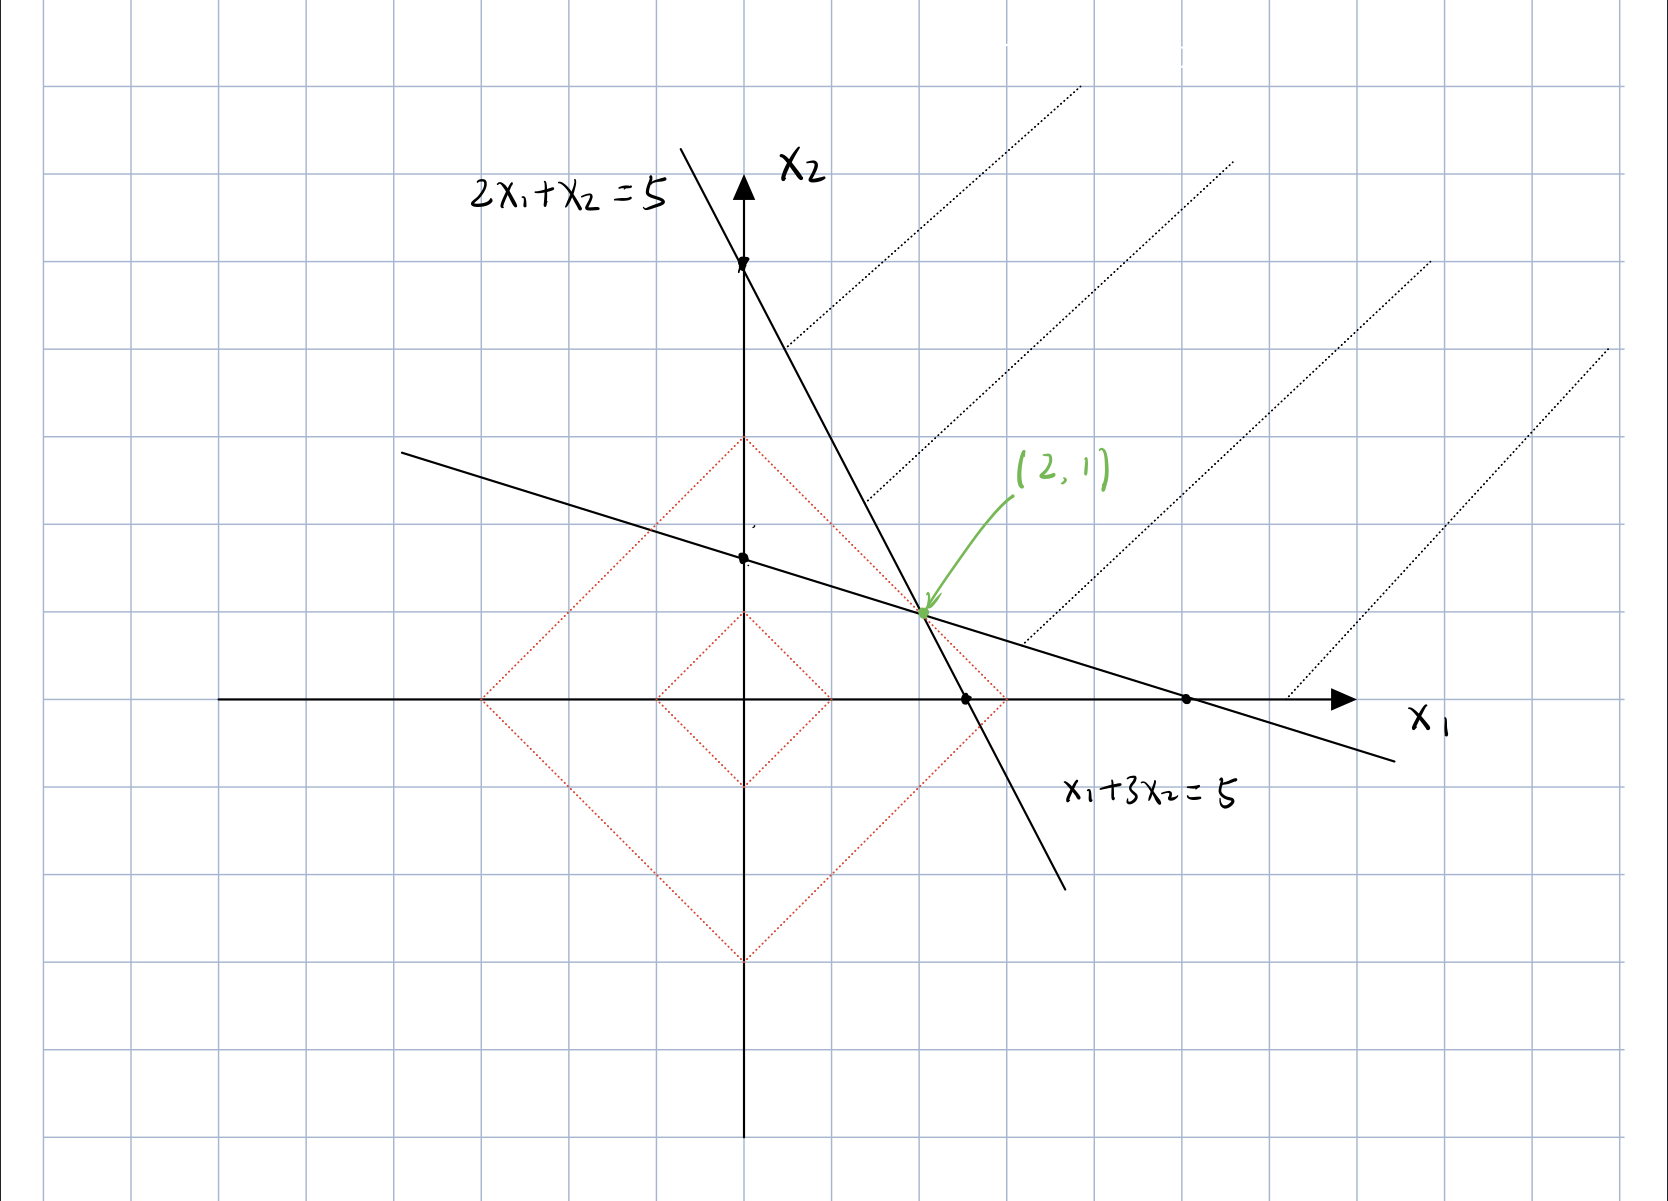
\includegraphics[width=.9\textwidth]{p4.jpeg}
		\caption{图解法}
	\end{figure}
	\end{itemize}
\end{enumerate}
	
\end{document} 